\section{Theoretische Grundlage}
\label{sec:Theorie}

\subsection{Ziel des Versuches}
In den folgenden Versuchen wird die Amplitude und der effektive Dämpfungswiderstand eines gedämpften Schwingkreises untersucht. Zusätzlich wird ermittelt bei welchem Widerstand der aperiodische Grenzfall eintritt. Zuletzt wird bei einer erzwungenen Schwingung die Frequenzabhängigkeit der Spannung und der Phasenverschiebung untersucht.

\subsection{Theorie}
Ein Schwingkreis besteht im Idealfall aus  einer Spule mit der Induktivität $L$ und einem Kondensator mit der Kapazität $C$, die in diesem System eingespeicherte Energiemenge wird immer wieder zwischen dem Kondensator und der Spule ausgetauscht. Während sich der Kondensator entlädt, entsteht in der Spule durch Induktion ein Magnetfeld. Sobald das Magnetfeld zusammenbricht wird der Kondensator wieder aufgeladen und der Vorgang beginnt erneut. \\
Anders ist das bei einem gedämpften oder realen Schwingkreis, da dieser noch einen Widerstand $R$ besitzt. Über diesen Widerstand wird laufend Energie in Wärme umgewandelt und geht entsprechend in dem Schwingkreis verloren. Daraus folgt das $R$ als Dämpfungsfaktor anzusehen ist.

\subsubsection{Differentialgleichung für die gedämpfte Schwingung}

\begin{figure}
	\centering
	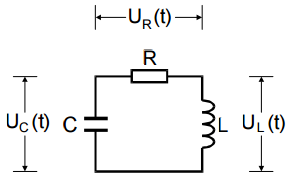
\includegraphics[height=4.5cm]{picture/Theorie1.PNG}
	\caption{Schematischer Aufbau eines RCL-Schwingkreises \cite[1]{sample}}
	\label{fig:RCL}
\end{figure}

Die in der Abbildung \ref{fig:RCL} eingezeichneten Spannungen $U_\text{R}$, $U_\text{C}$ und $U_\text{L}$ sind die Spannungen die über die entsprechenden Bauteile abfallen. Das zweite Kirchhoffsche Gesetzt besagt das alle Teilspannungen einer Masche sich zu null addieren, damit folgt:
\begin{equation}
	U_\text{R}(t) + U_\text{C}(t) + U_\text{L}(t) = 0 \ .
\end{equation}
Da nun
\begin{align*}
	U_\text{R}(t) &= R I(t) \ \ , \\
	U_\text{C}(t) &= \frac{Q(t)}{c} \ \ \ und \\
	U_\text{L}(t) &= L \frac{d I}{d t}
\end{align*}
ist, folgt mit weiteren umformungen
\begin{equation}
	\ddot{I}(t) + \frac{R}{L} \dot{I}(t) + \frac{1}{LC} I(t) = 0 \ .
\end{equation}
Die Differentialgleichung hat folgende Lösung:
\begin{equation}
	I(t) = e^{-2 \pi \mu t} \left(A e^{i2 \pi \nu t} + B e^{-i2 \pi \nu t} \right) \ ,
	\label{eqn:I}
\end{equation}
wobei die Abkürzungen
\begin{align*}
	\mu & := \frac{R}{4 \pi L} \\
	und \ \ \nu & := \frac{1}{2 \pi} \sqrt{\frac{1}{LC} - \frac{R^2}{4L^2}}
\end{align*}
verwendet wurden. \\
Im folgenden müssen nun zwei Fälle unterschieden werden.

\begin{table}
	\centering
	\begin{tabular}{c | c}
		erster Fall & zweiter Fall \\
		\midrule
		$\frac{1}{LC} < \frac{R^2}{4L^2}$ & $\frac{1}{LC} > \frac{R^2}{4L^2}$ \\
	\end{tabular}
\end{table}

\textbf{Erster Fall:} \\
Im reelen Fall, lässt sich Formel \ref{eqn:I} mit Hilfe der Eulerschen Formel zu
\begin{equation}
	I(t) = C e^{-2 \pi \mu t} \cos(2 \pi \nu t + \eta)
\end{equation}
umformen. Unter der genannten Bedingung ist zu erkennen das es sich um eine gedämpfte Schwingung handelt, die für $t \to \infty$ gegen Null strebt. Die Abklingdauer ist definiert als:
\begin{equation}
	T_\text{ex} = \frac{1}{2 \pi \mu} \ .
\end{equation}
Nach der Abklingdauer hat sich die Amplitude auf den e-ten Teil ihres ursprünglischen Wertes verringert.
\newline
\newline
\textbf{Zweiter Fall:} \\
Im imaginären Fall, kann Formel \ref{eqn:I}, nach einer hinreichend großen Zeit zu
\begin{equation}
	I(t) \propto e^{-(2 \pi \mu - i2 \pi \nu)t}
\end{equation}
umgeschrieben werden. \\
Von Bedeutung ist der Speziallfall:
\begin{align*}
	\frac{1}{LC} & = \frac{R_\text{ap}^2}{4L^2} \ \ \ \ \ d.h. \nu = 0 \ , \\
	dan&n \ wird \\
	I(t) & = C e^{- \frac{t}{\sqrt{LC}}} \ .
\end{align*}
Der Speziallfall stellt den aperiodischen Grenzfall dar, die Amplitude des Stromes fällt hier am schnellsten ab ohne über zu schwingen.

\subsubsection{Differentialgleichung für die erzwungene Schwingung}
In diesem Versuch wird ein von außen angeregter RCL-Schwingkreis untersucht. Dafür wird ein Sinusgenerator integriert. Der schematische Aufbau ist in Abbildung \ref{fig:aRCL} dargestellt.

\begin{figure}[H]
	\centering
	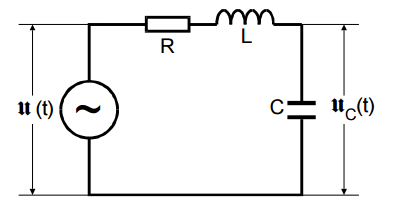
\includegraphics[height=4cm]{picture/Theorie2.PNG}
	\caption{Schematischer Aufbau eines angeregten RCL-Schwingkreises \cite[6]{sample}}
	\label{fig:aRCL}
\end{figure}

Die Differentialgleichung für dieses Problem ist nun inhomogen und lautet:
\begin{equation}
	LC \ddot{U}_\text{C}(t) + RC \dot{U}_\text{C}(t) + U_\text{C}(t) = U_0 e^{i \omega t} \ .
\end{equation}
Daraus folgt die Lösung für die Spannung zu:
\begin{equation}
	U = \frac{U_0(1 - LC \omega^2 - i \omega RC)}{(1 - LC \omega^2)^2 + \omega^2 R^2 C^2} \ .
\end{equation}
Die Phasenverschiebung ergibt sich aus dem Vergleich von Real- und Imaginärteil von $U$:
\begin{equation}
	\Phi (\omega) = \arctan \left(\frac{-\omega RC}{1-LC\omega^2}  \right)
\end{equation}
Es wird deutlich, dass sich die Frequenzen $\omega_1$ und $\omega_2$, bei denen die Phasenverschiebung die Werte $\frac{\pi}{4}$ bzw. $\frac{3\pi}{4}$ hat, zu
\begin{equation}
	\omega_{1,2} = \pm \frac{R}{2L} + \sqrt{\frac{R^2}{4L^2} + \frac{1}{LC}}
\end{equation}
ergeben.
Der Betrag von $U$ entspricht der gesuchten Lösungsfunktion $U_\text{C}(\omega)$, damit folgt:
\begin{equation}
	U_\text{C}(\omega) = |U| = \frac{U_0}{\sqrt{(1 - LC \omega^2)^2 + \omega^2 R^2 C^2}} \ .
	\label{eqn:Ucw}
\end{equation}
Es wird deutlich das $U_\text{C}(\omega)$ für $\omega \to \infty$ gegen Null strebt und für $\omega \to 0$ gegen $U_0$ strebt. Außerdem gibt es eine Frequenz bei der $U_\text{C}$ seinen Maximalwert erreicht, diese Frequenz wird Resonanzfrequenz genannt.
\begin{equation}
	\omega_\text{res} = \sqrt{\frac{1}{LC} - \frac{R^2}{2L^2}} \ .
\end{equation}
Wenn
\begin{align*}
	\frac{R^2}{2L^2} \ll \frac{1}{LC} \ ,
\end{align*}
dann wird von einer schwachen Dämpfung gesprochen. Es gilt $\omega_\text{res} \approx \omega_0$ wobei $\omega_0$ die Erregerfrequenz ist.
\begin{equation}
	\omega_0 = \sqrt{\frac{1}{LC}} \ .
\end{equation}
Die Güte des Schwingkreises lässt sich über:
\begin{equation}
	q = \frac{1}{\omega_0 RC}
\end{equation}
berechnen. Die maximale Spannung an dem Kondensator ist um den Faktor der Güte größer als die Erregerspannung. Es wird nun die Breite der Resonanzkurve betrachtet, welche duch \ref{eqn:Ucw} beschrieben wird. Wenn
\begin{align*}
	\frac{R^2}{L^2} \ll {\omega_0}^2
\end{align*}
berücksichtigt wird, folgt die Breite zu:
\begin{equation}
	\omega_+ - \omega_- \approx \frac{R}{L} \ .
\end{equation}
Die Güte folgt damit zu:
\begin{equation}
	q = \frac{\omega_0}{\omega_+ - \omega_-}
\end{equation}


\subsection{Fehlerrechnung}
Sämtliche Fehlerrechnungen werden mit Hilfe von Python 3.4.3 durchgeführt.
\subsubsection{Mittelwert}
Der Mittelwert einer Messreihe $x_\text{1}, ... ,x_\text{n}$ lässt sich durch die Formel
\begin{equation}
	\overline{x} = \frac{1}{N} \sum_{\text{k}=1}^\text{N} x_k
	\label{eqn:ave}
\end{equation}
berechnen. Die Standardabweichung des Mittelwertes beträgt
\begin{equation}
	\Delta \overline{x} = \sqrt{ \frac{1}{N(N-1)} \sum_{\text{k}=1}^\text{N} (x_\text{k} - \overline{x})^2}
	\label{eqn:std}
\end{equation}

\subsubsection{Gauß'sche Fehlerfortpflanzung}
Wenn $x_\text{1}, ..., x_\text{n}$ fehlerbehaftete Messgrößen im weiteren Verlauf benutzt werden, wird der neue Fehler $\Delta f$ mit Hilfe der Gaußschen Fehlerfortpflanzung angegeben.
\begin{equation}
	\Delta f = \sqrt{\sum_{\text{k}=1}^\text{N} \left( \frac{ \partial f}{\partial x_\text{k}} \right) ^2 \cdot (\Delta x_\text{k})^2}
	\label{eqn:var}
\end{equation}

\subsubsection{Lineare Regression}
Die Steigung und y-Achsenabschnitt einer Ausgleichsgeraden werden gegebenfalls mittels Linearen Regression berechnet.
\begin{equation}
	y = m \cdot x + b
	\label{eqn:reg}
\end{equation}
\begin{equation}
	m = \frac{ \overline{xy} - \overline{x} \overline{y} } {\overline{x^2} - \overline{x}^2}
	\label{eqn:reg_m}
\end{equation}
\begin{equation}
	b = \frac{ \overline{x^2}\overline{y} - \overline{x} \, \overline{xy}} { \overline{x^2} - \overline{x}^2}
	\label{eqn:reg_b}
\end{equation}
